\documentclass[a4paper,man,natbib]{apa6}

\usepackage[english]{babel}
\usepackage[utf8x]{inputenc}
\usepackage{amsmath}
\usepackage{graphicx}
\usepackage[colorinlistoftodos]{todonotes}

% override apa6 first paragraph index
% https://tex.stackexchange.com/questions/155028/indentation-apa6-class-for-2nd-paragraphs-after-title
% \makeatletter
%   \b@level@one@skip=-2.5ex plus -1ex minus -.2ex
%   \b@level@two@skip=-2.5ex plus -1ex minus -.2ex
% \makeatother

\title{Supplemental materials for ``An item response theory analysis of the Matrix Reasoning Item Bank (MaRs-IB)''}
\shorttitle{Supplemental materials for ``IRT analysis of MaRs-IB''}
\author{Samuel Zorowitz$^1$, Gabriele Chierchia$^3$, Sarah-Jayne Blakemore$^3$, Nathaniel D. Daw$^{1,2}$}
\affiliation{$^1$Princeton Neuroscience Institute, Princeton University, USA\\$^2$Department of Psychology, Princeton University, USA\\$^3$Department of Psychology, University of Cambridge, Downing Street, Cambridge, UK}

\setcounter{figure}{0}
\setcounter{table}{0}
\renewcommand{\thetable}{S\arabic{table}}
\renewcommand{\thefigure}{S\arabic{figure}}

\begin{document}
\maketitle

\section*{Speed-accuracy trade-offs in \cite{chierchia2019matrix}}

To investigate the possibility of speed-accuracy trade-offs in the MaRs-IB response data collected by \cite{chierchia2019matrix}, we looked at the proportion of correct responses to the easiest items (dimension 1 \& 2 items) as a function of the number of participants having reached that item. The logic is that, if items that appeared later in the fixed-order test were disproportionately reached by participants sacrificing accuracy for speed, then we should observe a positive correlation between the total number of available responses and proportion correct amongst the easiest items. 

We detected strong positive correlations between proportion correct and number reached (dimension 1 items: $\rho$ = 0.514, p = 0.050; dimension 2 items: $\rho$ = 0.767, p < 0.001; combined: $\rho$ = 0.695, p < 0.001). This result supports the hypothesis that participants that did reach items later in the test did so by prioritizing speed at the expense of accuracy. This suggests that the item summary statistics released as part of \cite{chierchia2019matrix} are likely biased indicators of item difficulty.

\section{Defining a threshold for rapid guessing}

In online testing environments, it is inevitable that some participants will not engage meaningfully with an experiment and instead in engage in careless or insufficient effort responding. On matrix reasoning tasks, one such low-effort strategy is rapid guessing wherein participants response in such a short time that there is no way they could have meaningfully considered an item \citep{wise2017rapid}. In sufficient quantities, the presence of rapid guesses in data can systematically bias estimates of item parameters. Thus, if possible, rapid guess responses should ideally be identified and removed. 

There are a number of approaches for identifying rapid guess responses (for a review, see \cite{wise2017rapid}). We opted for a threshold approach, in which responses taking less than a particular time would be denoted as rapid guesses and participants exhibiting too many rapid guessing responses would be excluded from the data. To define this threshold, we fit an extended version of the effort-moderated item response theory (EM-IRT) model \citep{wise2006application} to a small dataset of responses collected during piloting. In the EM-IRT, the probability of correct responding for participant $i$ to item $j$ is defined as the following mixture:

\begin{equation*}
    p(y_{i,j} = 1) = (1-w_{ij}) \cdot \gamma + w_{ij} \cdot \text{logit}^{-1} \left( \alpha_{j} \cdot \theta_i - \beta_{j} \right)
\end{equation*}

\noindent where $\theta_i$ is the latent ability for person $i$, and $\beta_{j}$, $\alpha_{j}$, and $\gamma_{j}$ are the difficulty, discrimination, and guessing parameters for item $j$. As in the main text, here we fixed the guessing parameter for every item clone to the nominal guessing rate ($\gamma_{j} = 0.25$). Crucially, $w_{ij}$ is a weight parameter, bounded between zero and one, that controls whether a participant is responding effortfully in accordance with their ability ($w_{ij} \rightarrow 0$) or engaging in rapid guessing responding ($w_{ij} \rightarrow 1$).

Here we defined the rapid guessing weight as a function of participant's response time on that trial:

\begin{equation*}
    w_{ij} = \text{logit}^{-1} \left( \zeta_0 + z_{ij} \cdot \zeta_1 + z_{ij}^2 \cdot \zeta_2 \right)
\end{equation*}

\noindent where $z_{ij}$ is the (log-transformed) response time for participant $i$ for item $j$, and  $\zeta_n$ are regressing coefficients mapping responses times to rapid guessing weights. Thus, this form of the EM-IRT model learns a function in a data-driven fashion to classify responses as having originated from effortful or rapid guessing response strategies. 

We fit this model to data collected from a total of N=180 participants recruited from the Prolific Academic platform during piloting. Each participant completed one of two sets of eight items from the MaRs-IB. The EM-IRT model estimated within a Bayesian framework using Hamiltonian Monte Carlo as implemented in Stan (v2.22) \citep{carpenter2017stan}. Four separate chains with randomised start values each took 3,000 samples from the posterior. The first 2,000 samples from each chain were discarded. As such, 4,000 post-warmup samples from the joint posterior were retained. The $\hat{R}$ values for all parameters were equal to or less than 1.01, indicating acceptable convergence between chains, and there were no divergent transitions in any chain.  

The estimated weights ($w_{ij}$) across all subjects and items are plotted as a function of their corresponding response time in Figure S2. As can be observed, the weights quickly approach 1 for response times faster than 5 seconds. Interestingly, weights begin to rise again for responses after 20 seconds suggesting that participants have an internal awareness of the amount of time that has elapsed.

To define a threshold for rapid guessing, we found the corresponding response time for which $w = 0.5$. This was at approximately 3 seconds. Thus, in the main experiments we defined rapid guessing as responses taking fewer than 3 seconds. 


\bibliography{supplement}

\begin{table}
    \centering
    \begin{tabular*}{0.45\textwidth}{ccr}
    \toprule
    Model & psis-loco & $\Delta$ psis-loco (se) \\
    \midrule
    1r & 28376.7 & 635.3 (29.7) \\
    1 & 27741.4 & \multicolumn{1}{c}{-} \\
    \midrule
    2r & 27627.6 & 665.6 (32.2) \\
    2 & 26962.1 & \multicolumn{1}{c}{-} \\
    \midrule
    3r & 27218.7 & 633.1 (33.9) \\
    3 & 26585.5 & \multicolumn{1}{c}{-} \\
    \bottomrule
    \end{tabular*}
    \caption{\label{tab:2}\normalfont Comparison of the first wave of item response models to their equivalents without a guessing parameter ($\gamma = 0$). LOO-CV values are presented in deviance scale (i.e. smaller values indicate better fit). Abbreviations: PSIS = Pareto-smoothed importance sampling; LOCO = leave-one-cluster-out.}
    \label{table:2}
\end{table}

\begin{table}
\centering
\begin{tabular*}{\textwidth}{ccccccllll}
\toprule
 & & & & & & \multicolumn{4}{c}{Spearman rank correlation} \\
\cmidrule(lr){7-10}
Measure & & Mean (SD) & & IQR & &  NFC-10 & PCF-8a & SNS & MaRs-SF \\
\midrule
NFC-10 & & 25.03 (8.27) & & 20.00 -- 31.00 & & \multicolumn{1}{c}{-} &  &  & \\
PCF-8a   &  & 22.17 (6.29) & & 18.75 -- 26.25 & & 0.27** &  \multicolumn{1}{c}{-} &  &  \\
SNS   &  & 29.07 (7.48) & & 25.00 -- 35.00 & & 0.46** &  0.29** &  \multicolumn{1}{c}{-} &   \\
MaRs-SF & &   8.00 (2.53) & &   6.00 -- 10.00 & & -0.04 &  0.04 &  0.14* &  \multicolumn{1}{c}{-} \\
\bottomrule
\end{tabular*}
\captionsetup{width=1.\textwidth}
\caption{\normalfont Correlations between performance on the MaRs-IB short forms and self-report measures. Abbreviations: IQR = interquartile range; NFC-10 = need for cognition (10-item) scale \citep{chiesi2018applying}; PCF = PROMIS cognitive functioning scale (8a; \citealt{iverson2021normative}); SNS = subjective numeracy scale \citep{fagerlin2007measuring}. ** p < 0.001,  * p < 0.05 (not corrected for multiple comparisons)}
\end{table}

\begin{figure}
\centering
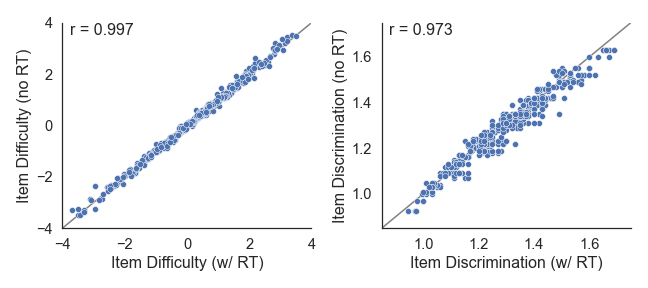
\includegraphics[width=1.0\textwidth]{figures/figS01.png}
\caption{\label{fig:figS01} An example item clone from each of the nine stimulus sets. In each row are three clones of one item template. Though some elementary shapes (e.g. circles, squares) are shared across stimulus sets, the majority of stimuli in each set are unique.}
\end{figure}

\begin{figure}
\centering
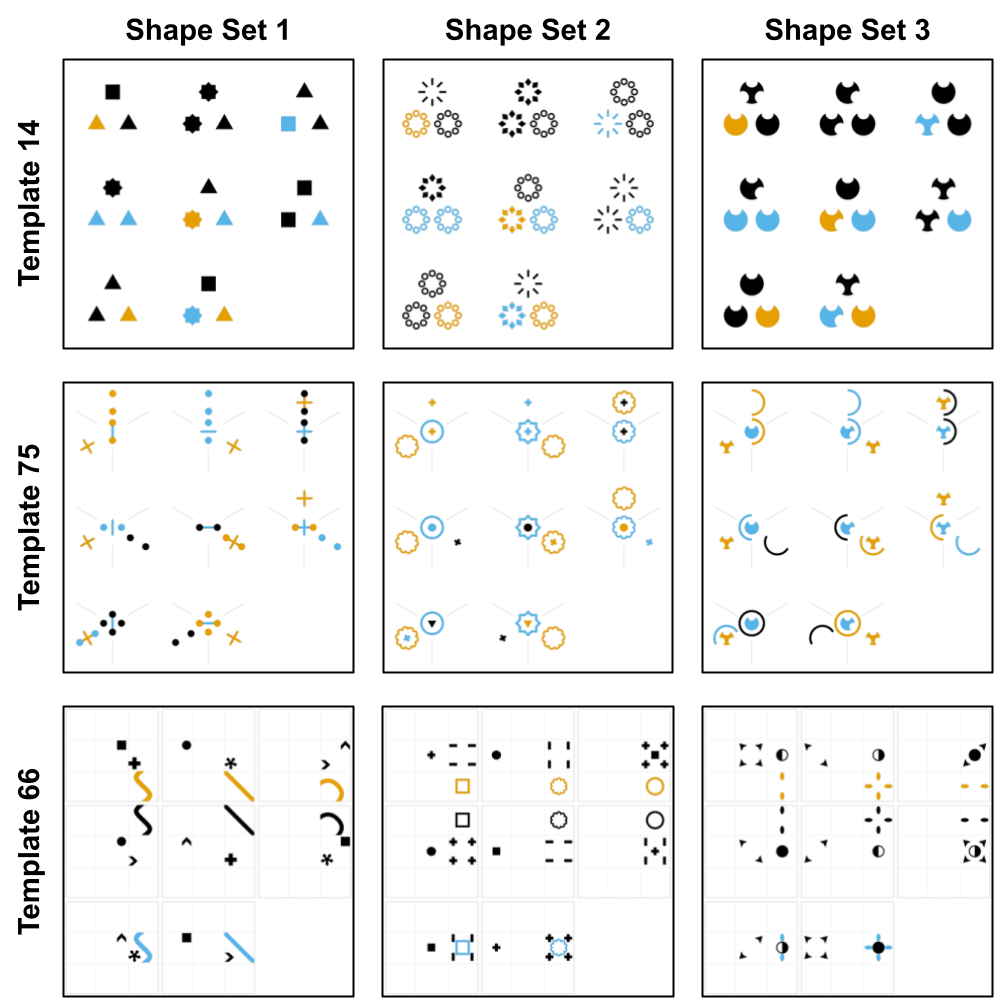
\includegraphics[width=0.8\textwidth]{figures/figS02.png}
\caption{\label{fig:figS02} Estimates of the rapid guessing weights ($w_{ij}$) and their corresponding responses times from the effort-moderated item response theory (EM-IRT) model fit to response data from N=180 pilot participants. The dashed line indicates the chosen rapid guessing threshold, i.e. where $w = 0.5$.}
\end{figure}

\end{document}